% VLDB template version of 2020-08-03 enhances the ACM template, version 1.7.0:
% https://www.acm.org/publications/proceedings-template
% The ACM Latex guide provides further information about the ACM template
%!TEX program = pdflatex
\documentclass[sigconf, nonacm]{acmart}

%% The following content must be adapted for the final version
% paper-specific
\newcommand\vldbdoi{XX.XX/XXX.XX}
\newcommand\vldbpages{XXX-XXX}
% issue-specific
\newcommand\vldbvolume{18}
\newcommand\vldbissue{1}
\newcommand\vldbyear{2025}
% should be fine as it is
\newcommand\vldbauthors{\authors}
\newcommand\vldbtitle{\shorttitle} 
% leave empty if no availability url should be set
%\newcommand\vldbavailabilityurl{https://github.com/Wangwenjing1996/Sirloin}
% whether page numbers should be shown or not, use 'plain' for review versions, 'empty' for camera ready
\newcommand\vldbpagestyle{plain}

\usepackage{subfigure}
\usepackage[vlined,ruled,linesnumbered]{algorithm2e}
\def\cmtb{\textcolor{blue}}
\def\cmtr{\textcolor{red}}
\usepackage{amsthm}
\usepackage{enumitem}
\usepackage{multirow}
\usepackage{balance}
\usepackage{flushend}
\usepackage{mdframed}
\usepackage{tcolorbox}
\usepackage{fancybox}

\newtheorem{example}{Example}
\newtheorem{definition}{Definition}
\newtheorem{lemma}{Lemma}
\newtheorem{theorem}{Theorem}
\newtheorem{remark}{Remark}

\newcommand{\E}{\mathrm{E}}
\newcommand{\Var}{\mathrm{Var}}

\newenvironment{summary}[1][]{\par\medskip
	\noindent\textbf{#1}
}{\medskip}

\newcounter{weakness}[section]
\setcounter{weakness}{0}
\renewcommand{\theweakness}{\arabic{weakness}}
\newenvironment{weakness}[1][]{\refstepcounter{weakness}\par\medskip
	\noindent\textbf{W\theweakness.#1} }{\medskip}

\newcounter{detailed}[section]
\setcounter{detailed}{0}
\renewcommand{\thedetailed}{\arabic{detailed}}
\newenvironment{detailed}[1][]{\refstepcounter{detailed}\par\medskip
	\noindent\textbf{D\thedetailed.#1} }{\medskip}

\newcounter{revision}[section]
\setcounter{revision}{0}
\renewcommand{\therevision}{\arabic{revision}}
\newenvironment{revision}[1][]{\refstepcounter{revision}\par\medskip
	\noindent\textbf{R\therevision.#1} }{\medskip}

\newcounter{metarevision}[section]
\setcounter{metarevision}{0}
\renewcommand{\themetarevision}{\arabic{metarevision}}
\newenvironment{metarevision}[1][]{\refstepcounter{metarevision}\par\medskip
	\noindent\textbf{R\themetarevision.#1} }{\medskip}

%\newcommand{\myfbox}[1]{%
%	\vspace{0.2cm}
%	\noindent
%	\fbox{\parbox{8.25cm}{#1}}
%	\vspace{0.15cm}
%}
\usepackage{xcolor}  % 确保引入了 xcolor 宏包

%\newcommand{\myfbox}[2][blue!5]{%
%	\vspace{0.2cm}
%	\noindent
%	\colorbox{#1}{\parbox{8.25cm}{#2}}%
%	\vspace{0.15cm}
%}

\newcommand{\myfbox}[1]{%
	\vspace{0.2cm}
	\noindent
	{\setlength{\fboxsep}{2.8pt}\setlength{\fboxrule}{0.4pt}%
		\fcolorbox{blue}{blue!6}{\parbox{8.25cm}{#1}}}%
	\vspace{0.15cm}
}

\begin{document}
%\title{Sirloin: Streaming Time Series Subsequence Anomaly Detection via Online Product Quantization}
\title{Response to Reviewer Comments:\\ ``
	An Experimental Evaluation of Hybrid Querying on Vectors (EA\&B)''\\
Submission to VLDB 2026 Research Track (ID )
}

\author{
	Jiaxu Zhu, Jiayu Yuan, Kaiwen Yang, Xiaobao Chen, Shihuan Yu, \\
	Hongchang Lv, Yan Li, Bolong Zheng
}
	
\maketitle
\pagestyle{plain}

\noindent
Dear meta-reviewer and reviewers:
	
Thank you for giving us the opportunity to revise our paper. We are deeply grateful for the reviewers' constructive feedback and the comprehensive suggestions provided in the meta-review. 
We believe that we have addressed all the major issues
and concerns, and the changes are highlighted \textcolor{blue}{in blue} according to the reviewers' comments.

\section*{Response To Meta-reviewer}

%%%%%%%%%%%%%%%%%%%% Summary %%%%%%%%%%%%%%%%%%%%
\myfbox{
	\begin{summary}[Summary Comments.]
		\textit{The paper empirically studies performance of hybrid querying methods with respect to two types of queries: attribute filtering (AF) NN search, range filtering (RF) NN search. This is a timely problem with high practical relevance. Nevertheless, several improvements would benefit the paper. We therefore recommend a revision. The main revision points are summarized below, however, we expect that the authors do their best in addressing all points raised in the individual reviews.}
	\end{summary}
}

\noindent
\textbf{Response:} 

%%%%%%%%%%%%%%%%%%%%%% R1 %%%%%%%%%%%%%%%%%%%%%%
\myfbox{
	\begin{metarevision}
		\textit{Improve the readability of some figures (e.g., performance under different attribute distributions or selectivity).}
	\end{metarevision}
}

\noindent
\textbf{Response:} We sincerely appreciate your valuable suggestions, which provide meaningful improvements to our work. Ensuring the readability of the figures is indeed crucial. We have modified both the figure and the related description in the paper to improve readability and ensure academic rigor. (Please see Section 4.2.3, highlighted in blue in the revised manuscript)

For performance under different attribute distributions, to illustrate how different algorithms are affected by varying attribute distributions, we added robustness indicators (Strong and Weak) in the figure. This provides more intuitive visualization of how robust each algorithm performs across different attribute distributions. As shown in Figure\ref{fig:attribute_distribution} below.

\begin{figure}[htbp]
	\centering
	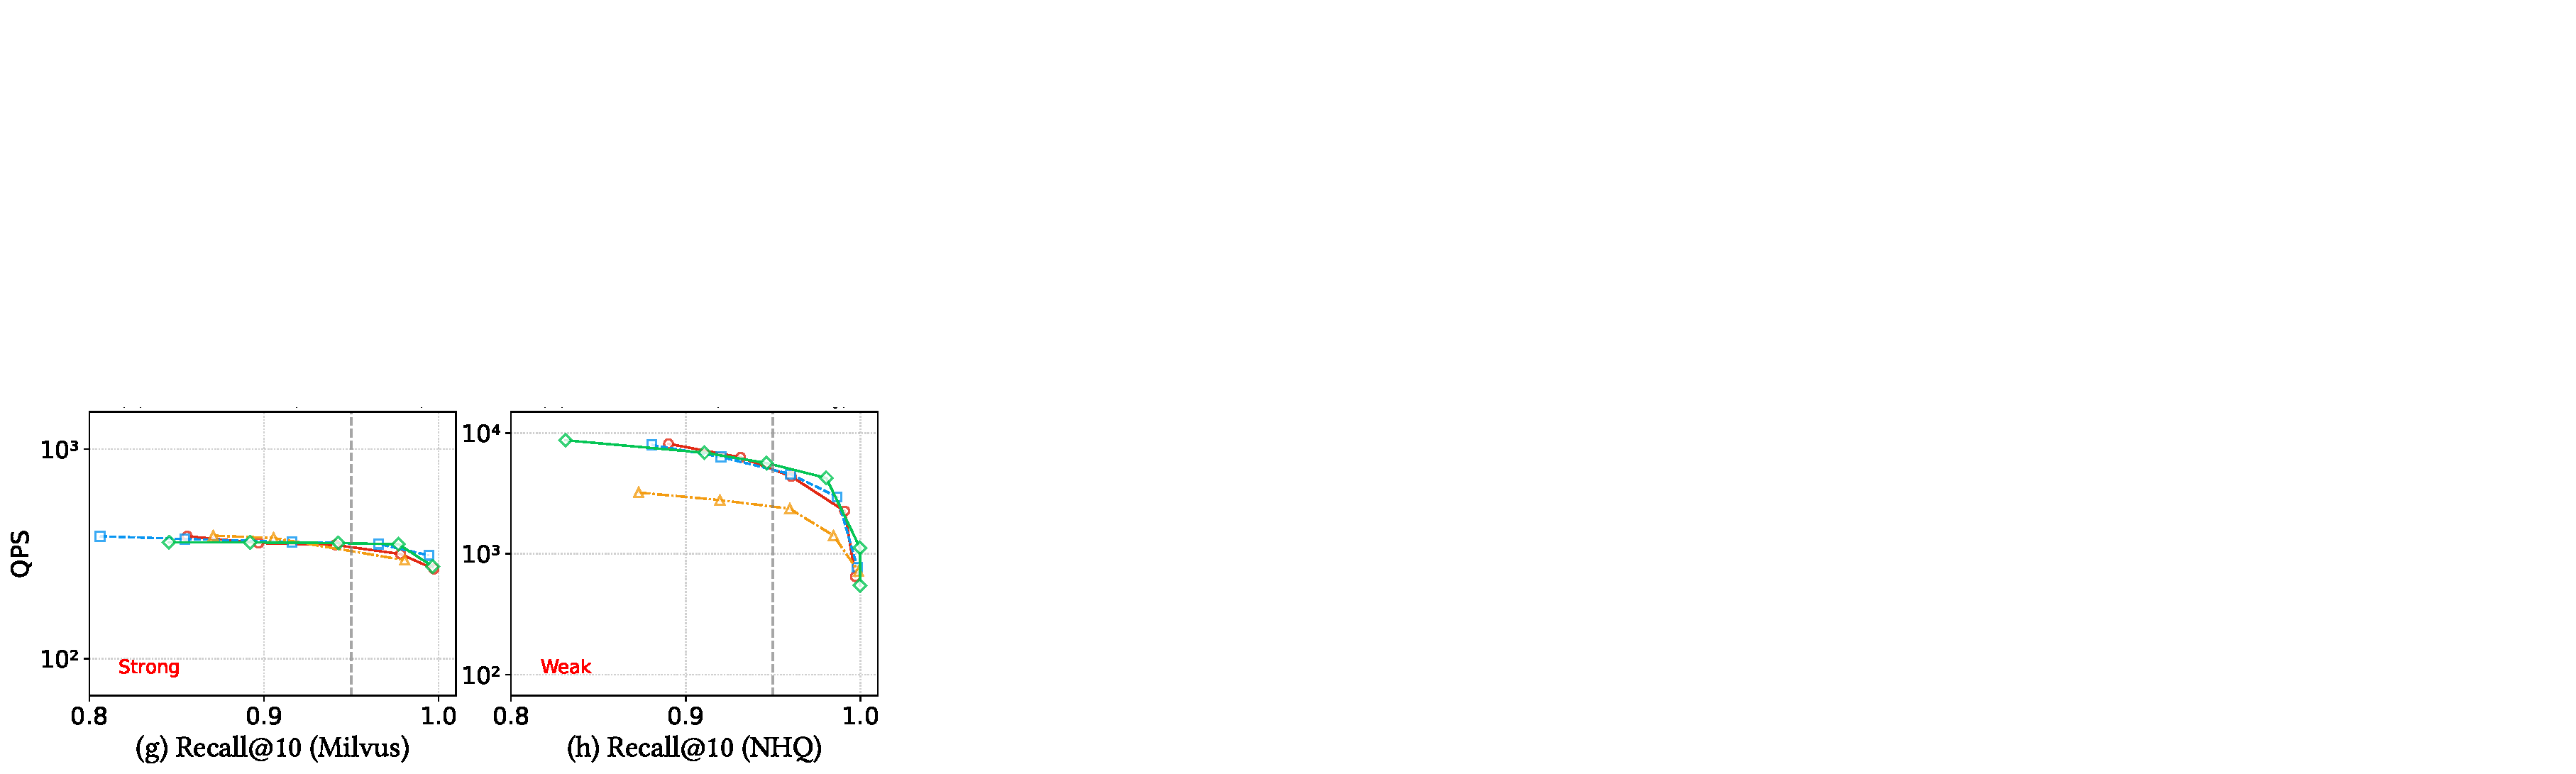
\includegraphics[width=\linewidth]{fig/exp_3_1.pdf}
	\caption{}
	\label{fig:attribute_distribution}
\end{figure}

For performance under different attribute selectivity, to reflect the performance differences of each algorithm under varying attribute selectivities, we added performance rankings for each algorithm across different selectivity levels in the figure. This provides a clearer illustration of how each algorithm is affected by attribute selectivity rates. As shown in Figure\ref{fig:attribute_selectivity} below.

\begin{figure}[htbp]
	\centering
	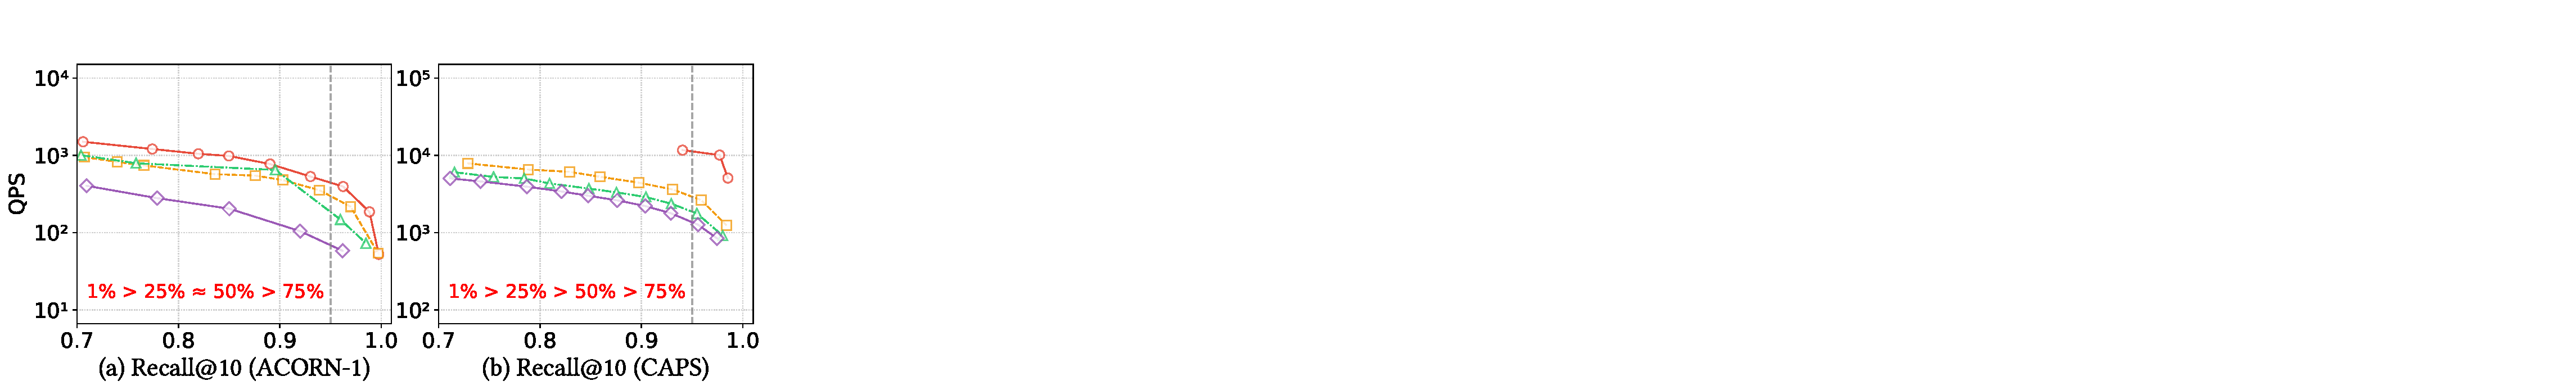
\includegraphics[width=\linewidth]{fig/exp_5_2_1.pdf}
	\caption{}
	\label{fig:attribute_selectivity}
\end{figure}

\textcolor{blue}{"The proximity of the 4 curves (representing different attribute distributions) in the figure reflects algorithm sensitivity to distributional variations. When the curves converge closely, the algorithm demonstrates strong resilience against attribute distribution shifts. Conversely, greater divergence among the curves indicates higher distributional dependence. Accordingly, the "Strong" label signifies robust performance consistency across varying distributions, while "Weak" denotes pronounced performance fluctuations under distributional changes."}

%%%%%%%%%%%%%%%%%%%%%% R2 %%%%%%%%%%%%%%%%%%%%%%
\myfbox{
	\begin{metarevision}
		\textit{Run experiments with multi-modal queries (e.g., combining text and images) or more complex query types involving both attribute and range filters.}
	\end{metarevision}
}

\noindent
\textbf{Response:} We believe this is an excellent suggestion. In fact, in the initial version of our paper, we use the text-to-image dataset that has been widely adopted by existing multimodal ANN algorithms. In this dataset, the base vectors are images, while the query set consists of texts, resulting in a modality gap between the two. Achieving good performance on such a dataset often requires the algorithm to demonstrate stronger robustness. \textbf{(Please refer to the last paragraph of Section 4.2.3 and the green highlighted part in Section 4.3.3.)}

To further enrich the evaluation of complex multimodal queries, we add new experiments in the Multi-modal Queries sections of Section 4.2.4 and Section 4.3.4. Specifically, we construct a more challenging multimodal dataset by selecting 500,000 text vectors and 500,000 image vectors as the base set, and 5,000 text vectors and 5,000 image vectors as the query set. We then perform both attribute filtering and range queries over this dataset, combining text and image queries to further analyze the robustness of the algorithms. The corresponding experimental results are presented in Section 4.2.4 and Section 4.3.4 under Multi-modal Queries.

As for complex query types that involve both attribute filtering and range queries simultaneously, to the best of our knowledge, existing algorithms—except for general-purpose systems such as Milvus and Faiss—do not support this functionality. For example, ACORN needs to build separate indexes for each scenario and cannot handle attribute filtering and range queries simultaneously. Therefore, we do not consider this type of complex query in our experiments but instead study the two query types separately. \textbf{(Please refer to the blue highlighted parts in Section 4.2.4 and Section 4.3.4 under Multi-modal Queries.)
}

\textcolor{blue}{
	"We conducted experiments on the text2image-mix dataset. This dataset contains both image and text vectors. It is a more complex multimodal dataset. As shown in Figure 12, although the queries are more complex, UNG and NHQ still perform the best. CAPS is the next best.
	Since the dataset mixes two modalities, the ground truth of the query set usually corresponds to the same modality. The nearest neighbors in the index are often from the same modality because they are closer in distance. Therefore, the search results on this dataset are similar to those in Figure 4. UNG and NHQ perform the best. CAPS clusters based on vector similarity. It actually clusters the vectors into the same modality. Then it uses attribute filtering to divide the data further. This allows CAPS to quickly find nearest neighbors that meet the filter conditions.
	In contrast, the text2image dataset shown in Figure 11 is different. The queries and the dataset are from different modalities. The queries are far from the dataset. The ground truths are also scattered and not clustered together. To find the ground truths, the algorithm often needs to traverse more points. This is a greater challenge for the algorithms." 
}

\textcolor{blue}{
		"Similar to attribute filtering, the performance of multimodal queries with range filtering shown in Figure 16a is also consistent with the single-modality results in Figure 14. As shown in Figure 15, the algorithms still perform the worst on multimodal datasets like Text2Image. This is because these range query algorithms are almost graph-based. Graph algorithms need more iterations to find true neighbors in OOD datasets."
}

%%%%%%%%%%%%%%%%%%%%%% R4 %%%%%%%%%%%%%%%%%%%%%%
\myfbox{
	\begin{metarevision}
		\textit{Instead of using the point ID, run experiments with meaningful attributes for RF-NN search on datasets (Deep, YT-Audio, WIT).}
	\end{metarevision}
}

\noindent
\textbf{Response:} 
Thank you for your suggestion. Using IDs as attributes for range filtering is a prevalent method in current range filtering algorithm evaluations, which indeed has considerable limitations. To address this issue, we add two datasets that use real attributes:

\textbf{YT-Audio-Real dataset:} For this dataset, we utilize the URLs provided by the YouTube8M dataset to crawl corresponding video categories and view counts as real attributes, using \textbf{video categories as attributes for attribute filtering experiments} and \textbf{view counts as attributes for range filtering experiments}, respectively.

\textbf{WIT-Real dataset:} We use the \texttt{clip-vit-base-patch32} model to encode the \texttt{page\_title} field from the WIT dataset into vectors, and extract the language type and the length of the \texttt{context\_page\_description} field as real attributes, applying them in both attribute filtering and range filtering experiments.

\textcolor{blue}{
	"Additionally, we introduced two datasets with real attributes for a more comprehensive evaluation of various attribute filtering and range query algorithms: The YT-Audio-Real dataset leverages URLs provided by the YouTube8M dataset to crawl corresponding video category IDs and view counts as its real attributes; whereas for the WIT-Real dataset, we used the \texttt{clip-vit-base-patch32} model to encode the \texttt{page\_title} field into vectors, and used the language type and the length of the \texttt{context\_page\_description} field as real attributes. It should be noted that, during range filtering, due to the limitations of some algorithms, we uniformly sorted the vectors according to the query attribute."
}
%%%%%%%%%%%%%%%%%%%%%% R5 %%%%%%%%%%%%%%%%%%%%%%


\myfbox{
	\begin{metarevision}
		\textit{Evaluate if the server setting affects the relative ordering of methods in experiments}
	\end{metarevision}
}

\noindent
\textbf{Response:} 
That is a great suggestion. In order to figure out if the server setting affects the relative ordering of methods, we conducted additional experiments on a server equipped with two Intel(R) Xeon(R) Gold 6330 CPUs @ 2.00GHz using the YT-Audio-Real dataset.
The results show that the performance differences across algorithms remain small, and their relative rankings do not change significantly across servers.
We did observe slightly lower QPS on this server compared to our original one, which is mainly due to the lower CPU frequency of the Xeon 6330 processors. Please see section 4.2.4.

\textcolor{blue}{"To investigate the impact of different server configurations on the performance of the algorithms, we conducted additional experiments on a server equipped with two Intel(R) Xeon(R) Gold 6330 CPUs @ 2.00GHz using the YT-Audio-Real dataset, and the results are shown in Figure 12(b). Compared with the experimental results on the original server (as shown in Figure 4d), the relative ranking of the algorithms remains largely unchanged, indicating that the performance of these methods is not significantly affected by differences in CPU configurations. Due to the lower CPU frequency of the Xeon 6330 compared to the original server, the QPS values are slightly lower across all methods."}

%%%%%%%%%%%%%%%%%%%%%% R6 %%%%%%%%%%%%%%%%%%%%%%
\myfbox{
	\begin{metarevision}
		\textit{In Table 1, please clarify which methods are disk-based, and which methods are memory-based.
			For disk-based methods, it is also meaningful to report the cost breakdown (e.g., in terms of I/O time and CPU time).}
	\end{metarevision}
}

\noindent
\textbf{Response:} 
Thank you for your suggestion. Currently, except for FilteredDiskANN, other hybrid query methods are memory-based, so we added the feature of whether to support disk for each algorithm in Table 1. At the same time, we also compared the search performance difference of FilteredDiskANN on memory and SSD using real data sets. The results are shown in Figure\ref{fig:recall-latency}:
\begin{figure}[htbp]
	\centering
	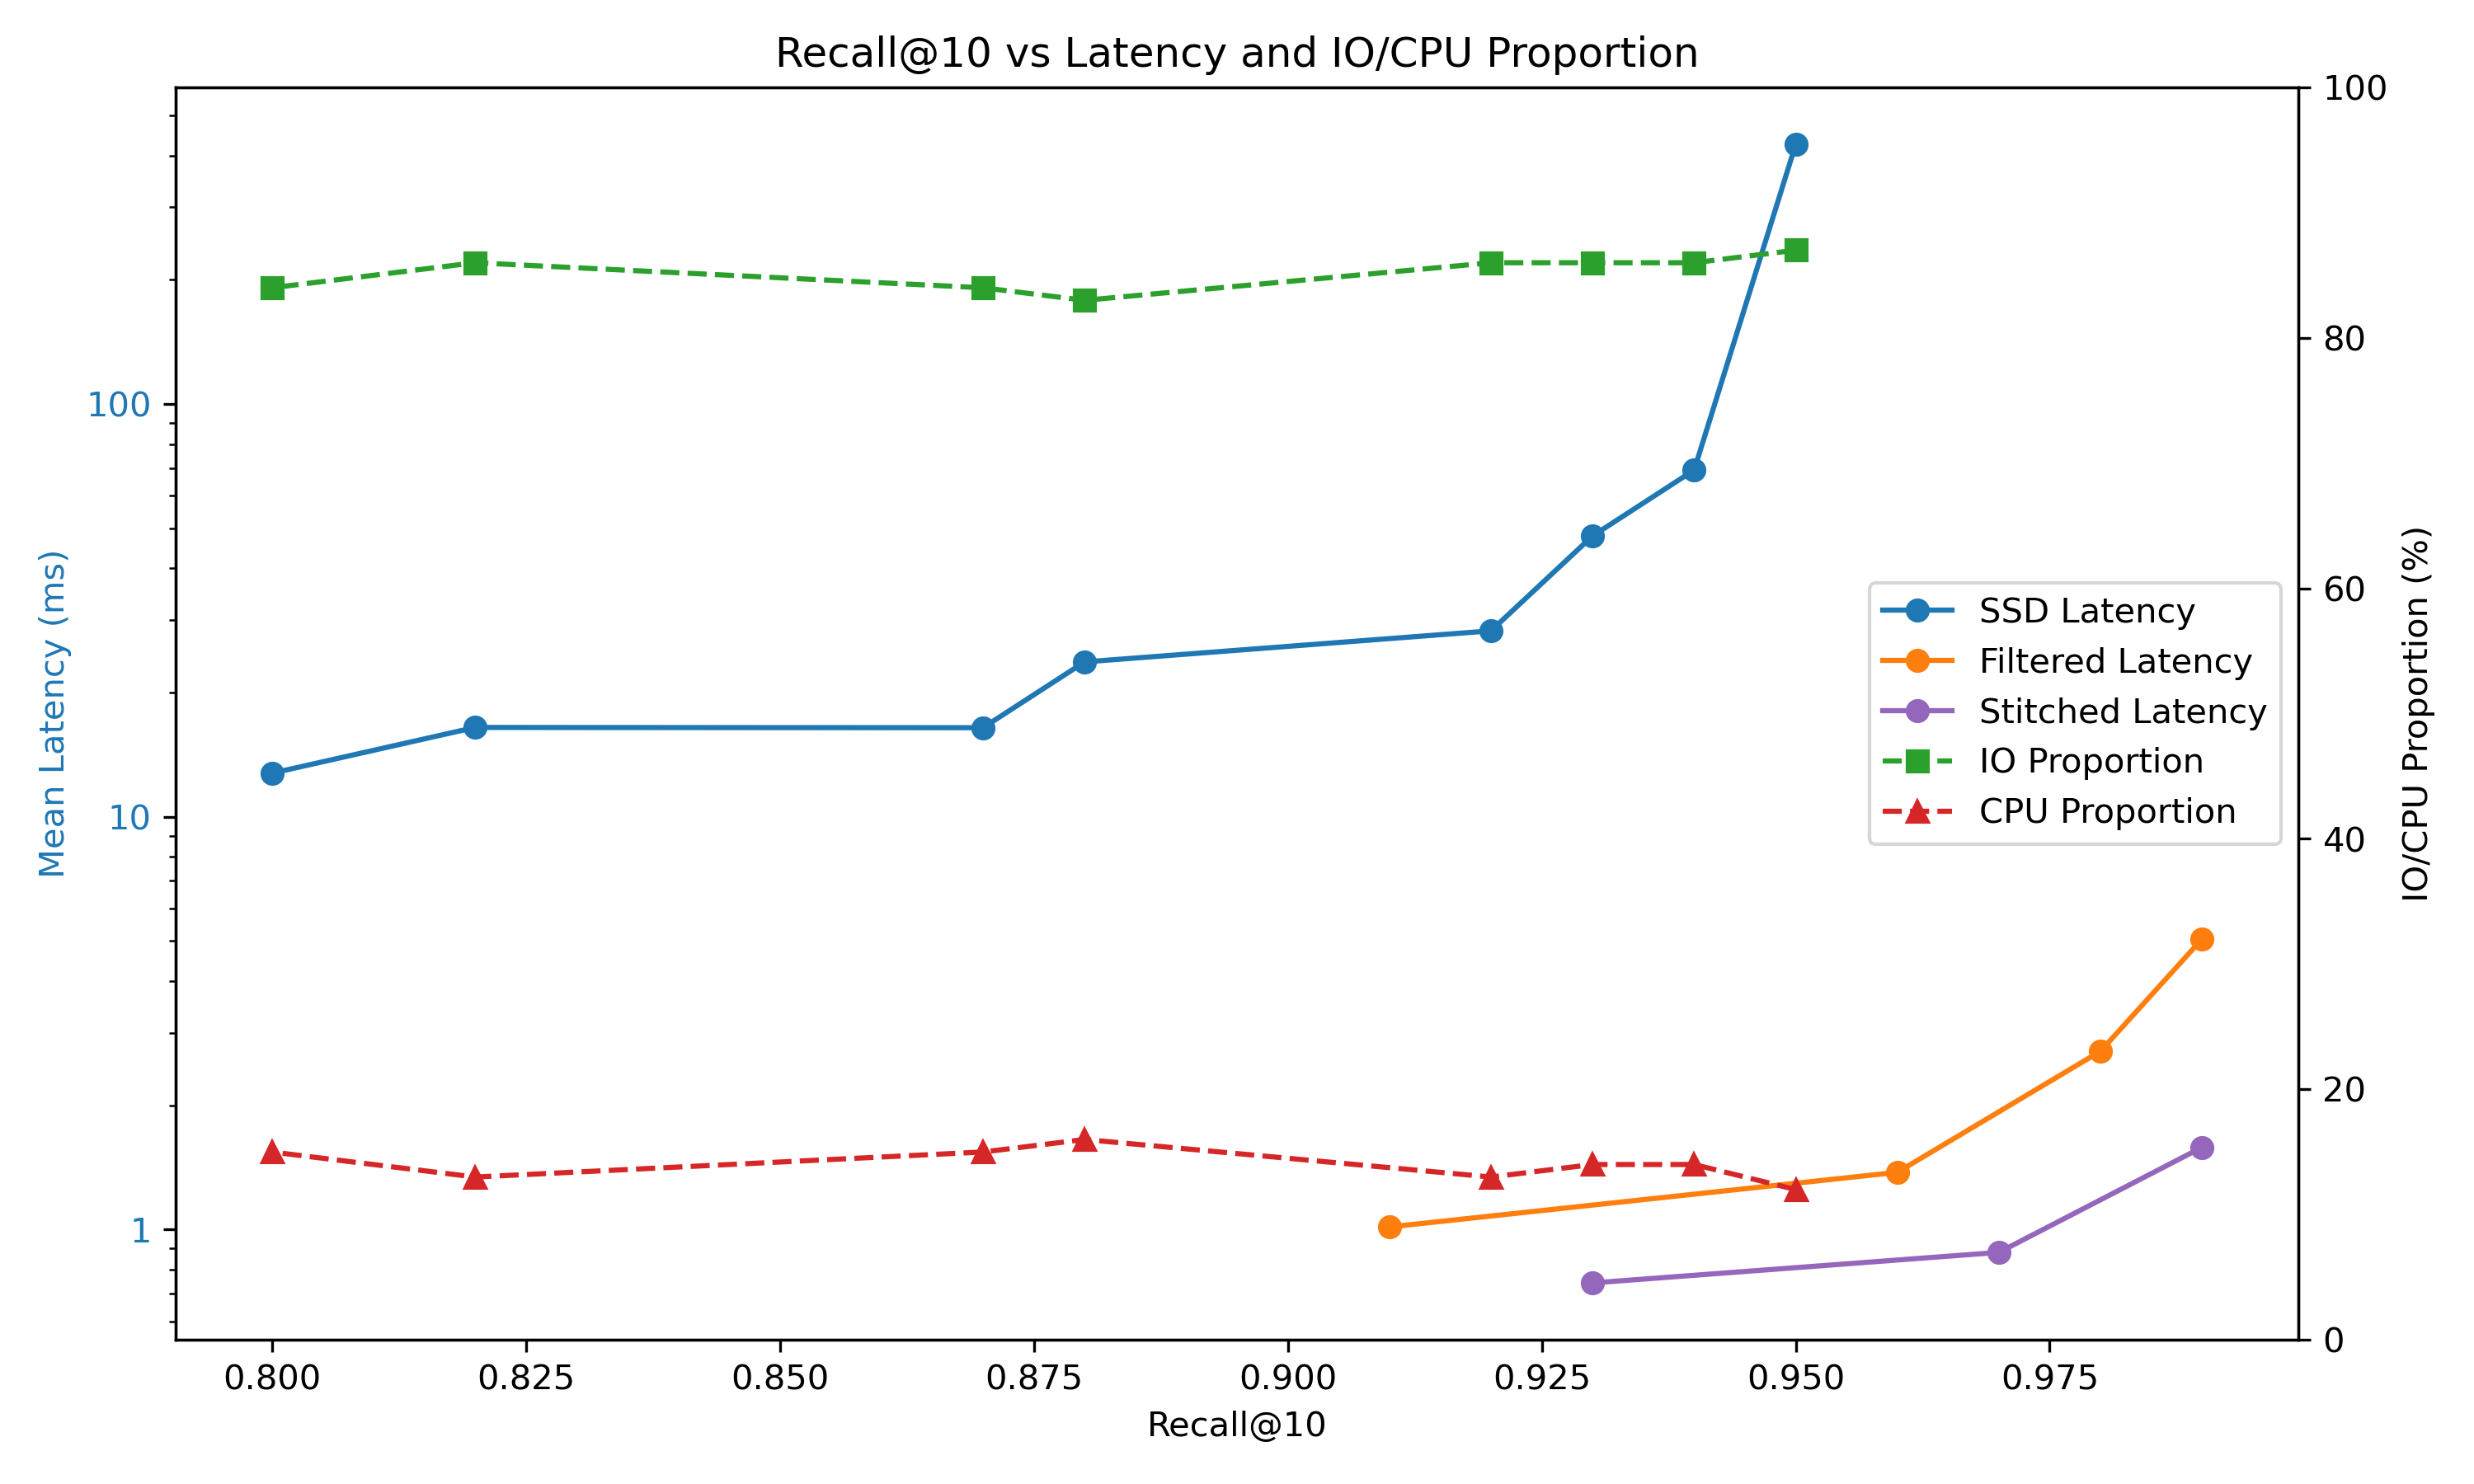
\includegraphics[width=\linewidth]{fig/recall_latency_all.png}
	\caption{}
	\label{fig:recall-latency}
\end{figure}

We conducted additional experiments on the real-world YT8M dataset, comparing three variants of DiskANN.
(1) SSD-based FilteredDiskANN (original disk-based method);
(2) FilteredVamana (memory-based method);
(3) StitchedVamana (memory-based method).


%\begin{itemize}
%	\item SSD-based FilteredDiskANN (original disk-based method)
%	\item FilteredVamana (memory-based method)
%	\item StitchedVamana (memory-based method)
%\end{itemize}


All experiments were run with 32 search threads for fair comparison. The following figure shows the mean latency (log-scale, left y-axis) and I/O vs CPU proportion (right y-axis) across different Recall\@10 levels:

\textbf{ Key Observations:}
Latency-Recall Tradeoff:
As expected, SSD-based FilteredDiskANN exhibits significantly higher latency than in-memory methods, especially at higher recall levels. When Recall@10 reaches 0.96, its latency increases super-linearly to over 100 ms.

Cost Breakdown of DiskANN:The I/O proportion consistently dominates, maintaining 80\%–85\% of the total latency even at different recall levels.
The CPU proportion remains low (10–15\%), indicating that I/O is the major bottleneck in disk-based search pipelines.
This clearly shows that improving disk read efficiency or reducing I/O volume is critical for performance optimization.

\textbf{In-memory Methods:}
FilteredVamana achieves a good balance, staying under 30 ms while achieving Recall@10 > 0.97.
While StitchedVamana achieves extremely low latency (sub-5 ms) due to its stitched multi-label index structure, its fixed edge connectivity may limit effectiveness under highly uncorrelated label distributions. Nevertheless, it consistently supports 90\%+ Recall@10 across diverse datasets, as shown in our evaluations.

\textbf{Note: }Due to space limitations and the fact that only one method supports disk-based execution, we did not include the above experiments and analysis in the revised paper.

%%%%%%%%%%%%%%%%%%%%%% R7 %%%%%%%%%%%%%%%%%%%%%%
\myfbox{
	\begin{metarevision}
		\textit{Report the peak memory usage of query processing.}
	\end{metarevision}
}

\noindent
\textbf{Response:} 
Thank you for your suggestion. We are deeply aware of this shortcoming, so we provide the search peak memory usage of each algorithm in the time and space overhead section and carefully analyze the reasons.
\begin{figure}[htbp]
	\centering
	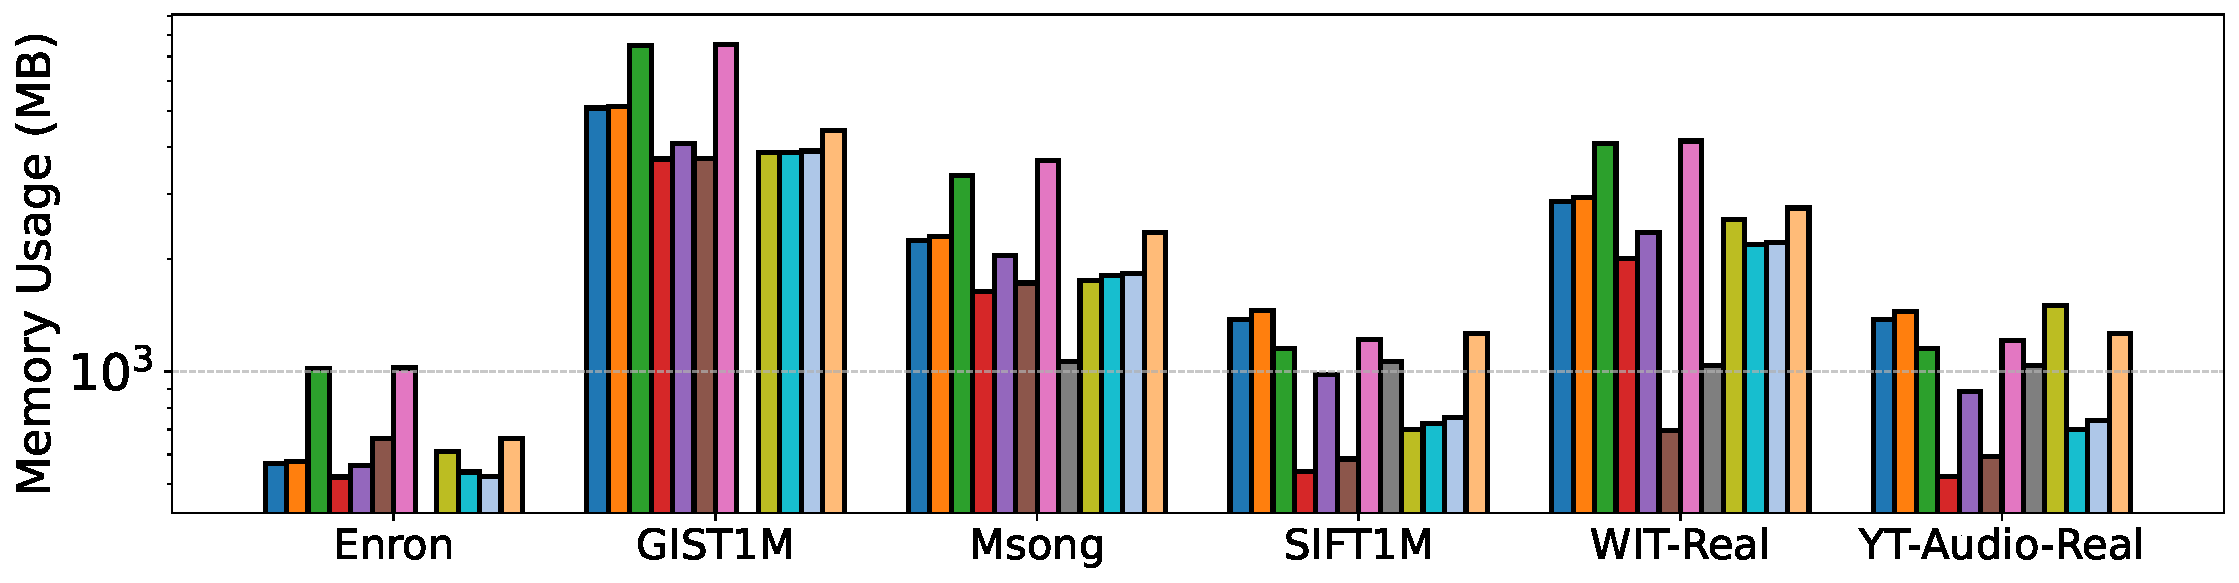
\includegraphics[width=\linewidth]{fig/searchMem/label_memory_comparison.pdf}
	\caption{attribute filtering search peak memory}
	\label{fig:attribute filtering search peak memory}
\end{figure}

\begin{figure}[htbp]
	\centering
	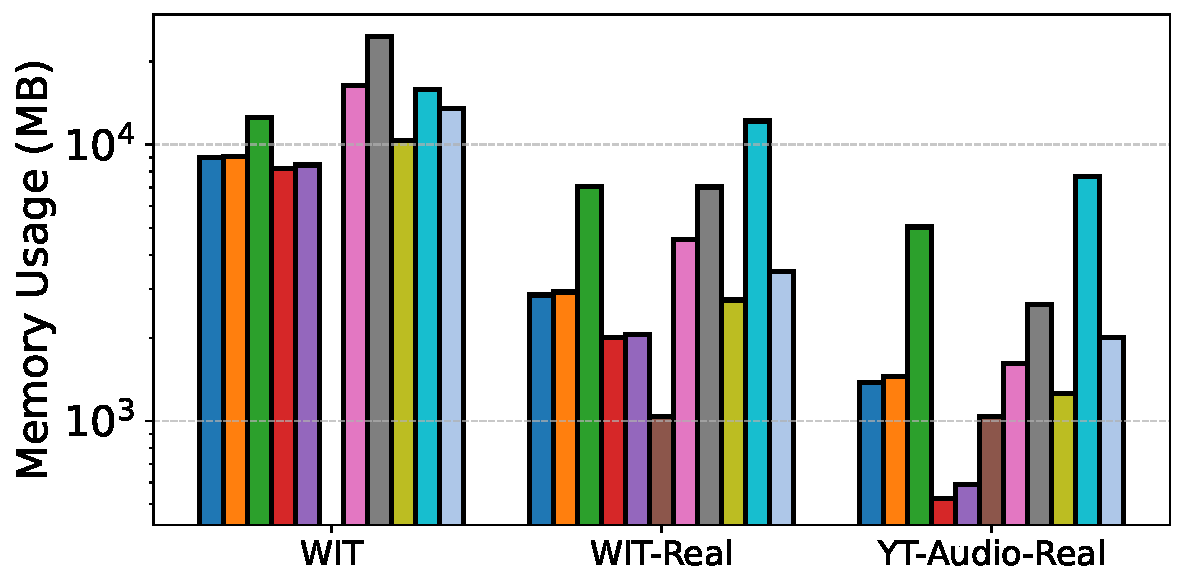
\includegraphics[width=\linewidth]{fig/searchMem/range_memory_comparison.pdf}
	\caption{range filtering search peak memory}
	\label{fig:range filtering search peak memory}
\end{figure}

For attribute filtering, please see section 4.2.1.

\textcolor{blue}{"As for the search peak memory usage, we can find from the Figure ~\ref{fig:attribute filtering search peak memory} that the peak memory usage of each algorithm during search does not differ significantly. Among them, CAPS and NHQ have relatively higher peak memory usage, while the peak memory usage of database is comparatively lower."}

For range filtering, please see section 4.3.1.

\textcolor{blue}{"As for the Search peak memory usage, we can find from the Figure ~\ref{fig:range filtering search peak memory} that it is basically consistent with the Build peak memory usage trend. The algorithm needs to load the complete index into memory during search. Therefore, algorithms with high building overhead, such as WinFilter, also have high search overhead; algorithms with low building overhead, such as Faiss, also have low search overhead. For Milvus, search does not require full index loading and there is additional metadata overhead when building, so the performance is different from the trend."}


%%%%%%%%%%%%%%%%%%%%%% R8 %%%%%%%%%%%%%%%%%%%%%%
\myfbox{
	\begin{metarevision}
		\textit{Run Scalability experiments with larger datasets.}
	\end{metarevision}
}

\noindent
\textbf{Response:} 
Thank you for your valuable suggestion regarding our experiments. In Section 4.2.4 and Section 4.3.4, we add experiments on the Deep100M dataset. The results show that most algorithms struggle to balance performance with time and space costs on this large-scale dataset. In particular, StitchedVamana performs poorly on Deep100M. For attribute filtering, please see section 4.2.4.

\textcolor{blue}{"On the 100M dataset, UNG and NHQ still exhibit excellent performance, demonstrating their good adaptability to large-scale datasets; however, this also comes with significant memory overhead. The clustering-based algorithm \texttt{Faiss+HQI\_Batch} shows moderate performance but has very low memory overhead, which makes it highly attractive for practical applications. We did not present the experimental results for StitchedVamana because we found that its recall consistently remained at a very low level. Its search starting point is set to 0 by default, and when the entry point is far from the target area, it easily gets stuck in a local optimum, making it difficult to navigate to the vicinity of the correct point."}

For range filtering, please see section 4.3.4.

\textcolor{blue}{"As shown in the figure 16c, in the 100-million-scale dataset, the top 3 ranked algorithms (WinFilter, UNIFY, and iRange) remain unchanged. However, their high performance is achieved at the cost of extremely high memory consumption (300-400GB). At the same time, we can see that some algorithms (e.g., SeRF, ACORN-1) perform even worse than the VBASE database, which indicates that they do not adapt well to large-scale dataset scenarios. Although Milvus has a low QPS, it can achieve a recall of 1 with an excellent memory footprint of around 80GB"}

%%%%%%%%%%%%%%%%%%%%%% R9 %%%%%%%%%%%%%%%%%%%%%%
\myfbox{
	\begin{metarevision}
		\textit{Clearer insights and guidelines wrt the strength and weaknesses of the compared system.}
	\end{metarevision}
}

\noindent
\textbf{Response:} 
Thank you for your valuable suggestion. We agree that our previous analysis of the strengths and weaknesses of the algorithms was not sufficiently clear.

To address this, we add a summary table that provides a clearer and more structured comparison of the strengths and weaknesses of each algorithm, offering deeper insights and more concrete guidelines for understanding their trade-offs.
%下面放那个优劣势表

%%%%%%%%%%%%%%%%%%%%%% R10 %%%%%%%%%%%%%%%%%%%%%%
\myfbox{
	\begin{metarevision}
		\textit{Clearer guidelines in the Discussion to the extend of recommendations on which system/algo to use for what dataset characteristics.}
	\end{metarevision}
}

\noindent
\textbf{Response:} 


\section*{Response to Review 1}

%%%%%%%%%%%%%%%%%%%%%% W1 %%%%%%%%%%%%%%%%%%%%%%
\myfbox{
	\begin{weakness}
		\textit{Although the authors justify the synthetic attribute generation, real-world applications may involve more complex attribute semantics and correlations, which might affect generalizability.}
	\end{weakness}
}

\noindent
\textbf{Response:} I really appreciate your suggestion. In real-world applications, vectors and their attributes often have complex relationships. To better reflect such scenarios, we have introduced two real-world datasets, which are described in detail in Meta-Review R3.
Interestingly, our results indicate that using real attribute values has limited impact on the overall performance trends.(Please see the experimental results in Section 4.2.2 and Section 4.3.2)

Regarding the more intricate semantic relationships—such as those between vectors and attributes, or among different attributes themselves—current hybrid search algorithms do not explicitly model or leverage such correlations. Nevertheless, our evaluation covers a range of realistic scenarios, including multi-attribute settings and diverse  distributions, to assess the generalization ability of the algorithms.

%%%%%%%%%%%%%%%%%%%%%% W2 %%%%%%%%%%%%%%%%%%%%%%
\myfbox{
	\begin{weakness}
		\textit{Some figures (e.g., performance under different attribute distributions or selectivity) are dense and could benefit from cleaner presentation or summarization to improve readability.}
	\end{weakness}
}

\noindent
\textbf{Response:} 
Thank you for your feedback. We improve the readability of the two figures in Section 4.2.3, and please see Meta-Review R1 for details. 


%%%%%%%%%%%%%%%%%%%%%% W3 %%%%%%%%%%%%%%%%%%%%%%
\myfbox{
	\begin{weakness}
		\textit{It would strengthen the paper to delve into multi-modal queries (e.g., combining text and images) or more complex query types involving both attribute and range filters.}
	\end{weakness}
}

\noindent
\textbf{Response:} 
Thank you for your suggestion. We have addressed this issue in detail in our response to Meta-Review R2. Specifically, we add complex multimodal query experiments and provided an in-depth analysis of the results. For more details, please refer to our response to Meta-Review R2.
%We think this is an excellent suggestion. We have enhanced our experiments by incorporating more complex multimodal dataset evaluations in Section \textcolor{blue}{XXX} of the paper. Initially, our paper utilized the Text2Image dataset, which is commonly used in existing multimodal ANN algorithms. This dataset presents a modality gap, as the base vectors are images while the query set consists of text, often requiring algorithms to exhibit stronger robustness for good performance. To further enrich the evaluation of complex multimodal queries, we selected 500,000 text vectors and 500,000 image vectors from the Text2Image dataset to form a mixed base query dataset. Similarly, we chose 5,000 image vectors and 5,000 text vectors as query vectors, combining both text and image modalities. We then performed attribute filtering and range queries on this multimodal dataset to further analyze algorithm robustness.  The relevant experimental results are presented and discussed in Section\textcolor{blue}{XXX}of our paper.

\section*{Response to Review 2}
\setcounter{weakness}{0}

%%%%%%%%%%%%%%%%%%%%%% W1 %%%%%%%%%%%%%%%%%%%%%%
\myfbox{
	\begin{weakness}
		\textit{In the experimental study, datasets did not originate from the real applications for hybrid queries.
			Regarding the datasets for AF-NN search (Msong, Audio, SIFT1M, GIST1M, GloVe, Enron),
			the attributes were generated synthetically but not real.
			Regarding the datasets for RF-NN search (Deep, YT-Audio, WIT), the data point ID was used as attribute;
			however, it is not meaningful to issue range query on data point ID.
			In order to match with the introduction, the authors are recommended to
			include a real dataset from e-commerce platform with both vectors and attributes.
		}
	\end{weakness}
}




\noindent
\textbf{Response:} 
Thank you for your suggestion. We fully understand your concern regarding the use of synthetic or less meaningful attributes in our hybrid query experimental setup.

To address this crucial issue and enhance the real-world relevance of our evaluation, we have added two new real-world datasets with genuine attributes to our attribute filtering and range query experiments, as detailed in MetaReview R3.

We have revised the manuscript accordingly. (Please see page 7, Section 4.2.1, and the "Single-Attribute Building and Single-Attribute Query" subsection of Section 4.2.2 on page 8, highlighted in blue in the revised manuscript.) Furthermore, it should be noted that, in the "Single-Attribute Building and Single-Attribute Query" subsection of Section 4.2.2 on page 8, due to space constraints, we have removed two previous datasets (Audio and GloVe), as Audio is relatively small-scale, and GloVe's scale is similar to SIFT1M while its LID is similar to GIST1M.

%%%%%%%%%%%%%%%%%%%%%% W2 %%%%%%%%%%%%%%%%%%%%%%
\myfbox{
	\begin{weakness}
		\textit{All experiments were conducted on the same server mentioned in Section 4.1.3.
			However, in practice, server providers may use other hardware settings (with other processors and RAM).
			Would the server setting affect the relative ordering of methods in experiments?
			For example, if Intel Xeon processor is used, would there be any change of the top 3 methods in Figures 4,5,7,8?
			Would the CPU cache size affect the top 3 methods in those figures?}
	\end{weakness}
}



\noindent
\textbf{Response:} 
Thank you for your suggestion. We add relevant experiments conducted on different servers in Section 4.2.4. Please refer to the response MR.R4 for more details.
%%%%%%%%%%%%%%%%%%%%%% W3 %%%%%%%%%%%%%%%%%%%%%%

\myfbox{
	\begin{weakness}
		\textit{In the experimental setup, it is unclear whether data storage (disk or SSD) is used.
			In Table 1, please clarify which methods are disk-based, and which methods are memory-based.
			For disk-based methods, it is also meaningful to report the cost breakdown (e.g., in terms of I/O time and CPU time).}
	\end{weakness}
}

\noindent
\textbf{Response:} 
Thank you for your suggestion. We have made a detailed response to this question in R5 of Response To Meta-reviewer. Please see R5 for details.


%%%%%%%%%%%%%%%%%%%%%% W4 %%%%%%%%%%%%%%%%%%%%%%
\myfbox{
	\begin{weakness}
		\textit{The authors have reported the peak memory usage of index construction only.
			They are also recommended to report the peak memory usage of query processing.}
	\end{weakness}
}

\noindent
\textbf{Response:} 
Thank you for your suggestion. We have made a detailed response to this question in R6 of Response To Meta-reviewer. Please see R6 for details.
	
%%%%%%%%%%%%%%%%%%%%%% D1 %%%%%%%%%%%%%%%%%%%%%%
\myfbox{
	\begin{detailed}
		\textit{The authors have cited an experimental paper [49],
			but have not discussed about the main difference between their paper and [49].}
	\end{detailed}
}



\noindent
\textbf{Response:} 
Thank you for pointing this out. Both paper [49] and our paper are benchmarks. Paper [49] provides a comprehensive review and evaluation of graph-based approximate nearest neighbor search algorithms. Our paper is the first benchmark to evaluate hybrid queries. Since hybrid queries are developed based on ANN, we refer to the evaluation metrics proposed in the cited paper. We realize that we did not clearly explain the difference between our paper and the cited paper, so we add a description in the introduction, please see section XXX.
\textcolor{blue}{""}



%%%%%%%%%%%%%%%%%%%%%% D2 %%%%%%%%%%%%%%%%%%%%%%
\myfbox{
	\begin{detailed}
		\textit{In Section 1.1, I could not find convincing references for the requirements in practical applications.
			[12] and [36] are research papers only, but not from real applications.}
	\end{detailed}
}


\noindent
\textbf{Response:} 
Thank you for your suggestion. We cited these two papers in the introduction to show that there are several papers that study attribute distribution and selectivity.
In addition, attribute distribution and selectivity are indeed widely used in real-world scenarios. For attribute distribution, the label attributes of many recommendation application scenarios in reality conform to the power-law distribution. For attribute selectivity: For example, if you need to query data with a very small proportion of a certain attribute, choosing a better algorithm will greatly improve the search effect. There are also some databases with practical applications that mention attribute selectivity, such as Milvus and AnalyticDB-V. For the two parts you suggested, we will add more comprehensive references in the paper.

Please see section 1.1. 

\textcolor{blue}{"For attribute filtering algorithms, factors such as the number of attributes, attribute distribution[12], and attribute  selectivity [46,51] significantly impact algorithm performance."}

%%%%%%%%%%%%%%%%%%%%%% D3 %%%%%%%%%%%%%%%%%%%%%%
\myfbox{
	\begin{detailed}
		\textit{In Definition 2.3, $ s_1 $ and $ s_n $ should be replaced with $ a_1 $ and $ a_n $ , respectively.}
	\end{detailed}
}


\noindent
\textbf{Response:} 
Thank you for pointing it out. We sincerely apologize for the misuse of notation in Definition 2.3. This has been corrected in the revised version. (Please see Definition 2.3 in Section 2.1, highlighted in blue in the revised manuscript)

\textcolor{blue}{"Let \( D = \{(v_1, a_1), \ldots, (v_n, a_n)\} \) be a dataset of \( n \) \( d \)-dimensional vectors, each associated with an attribute value \( a_i \)."}

%%%%%%%%%%%%%%%%%%%%%% D4 %%%%%%%%%%%%%%%%%%%%%%
\myfbox{
	\begin{detailed}
		\textit{ In Section 4.1, please clarify the URL of the implementation of each method.}
	\end{detailed}
}


\noindent
\textbf{Response:} 
Thank you for the suggestion. Since there are multiple methods, listing all URLs in Section 4.1 would be overwhelming. Instead, in Section 3, we add superscript markers next to each algorithm name and provide the corresponding implementation URLs as footnotes on the same page. (Please see the relevant footnotes in Section 3 in the revised manuscript)






\section*{Response to Review 3}
\setcounter{weakness}{0}

%%%%%%%%%%%%%%%%%%%%%% W1 %%%%%%%%%%%%%%%%%%%%%%
\myfbox{
	\begin{weakness}
		\textit{Scalability experiments are missing; largest dataset is 10M; some pitfalls will only show at large scale.}
	\end{weakness}
}


\noindent
\textbf{Response:} 
Thank you for your suggestion. We add experiments on the Deep100M dataset in Section 4.2.4 and Section 4.3.4, and we observe some pitfalls. For more details, please refer to our response to Meta Review R7.

%%%%%%%%%%%%%%%%%%%%%% W2 %%%%%%%%%%%%%%%%%%%%%%
\myfbox{
	\begin{weakness}
		\textit{The explanations provided with the performance results are not as insightful as they need to be to point out the pros and cons of the different algorithms.}
	\end{weakness}
}

\noindent
\textbf{Response:} 
Thank you for pointing this out. We agree that the initial explanations accompanying the performance results were not sufficiently detailed in highlighting the strengths and weaknesses of the compared algorithms. We conduct a more in-depth analysis of the reasons behind certain behaviors observed in the experimental results. The specific revisions are as follows:
%下面写每个修改过的理由
%%%%%%%%%%%%%%%%%%%%%% W3 %%%%%%%%%%%%%%%%%%%%%%

\myfbox{
	\begin{weakness}
		\textit{I'd expect general, clearer guidelines in the Discussion to the extend of recommendations on which system/algo to use for what dataset characteristics. Hence, the comprehensive perspective on their strengths and weaknesses of the approaches is missing.}
	\end{weakness}
}




\noindent
\textbf{Response:} 

\setcounter{detailed}{0}

%%%%%%%%%%%%%%%%%%%%%% D1 %%%%%%%%%%%%%%%%%%%%%%
\myfbox{
	\begin{detailed}
		\textit{Section 2.2. Graph based and IVF are well known. Missing in the index description is the implementation of attributes for AF and RF as the section is call hybrid ANN.}
	\end{detailed}
}



\noindent
\textbf{Response:}
Thank you for your suggestion. We acknowledge that the original manuscript did not clearly explain how attribute filtering (AF) and range filtering (RF) are embedded into standard graph-based and IVF-based index structures. We revise Section 2.2 and add two paragraphs. These paragraphs summarize how the algorithms discussed in this paper implement hybrid query functionality based on these foundational indexing structures.

\textcolor{blue}{"Graph-based indexes are widely adopted in Hybrid ANN search algorithms due to their excellent performance. To support hybrid queries, existing approaches usually augment the original graph structures by explicitly associating attribute or range information with vertices or edges. In attribute filtering, a common approach is to attach attribute metadata to vertices or edges, allowing the traversal process to skip nodes or edges that do not meet the query's attribute conditions (e.g., NHQ, Filtered-DiskANN, ACORN). In range filtering, edges typically store valid attribute intervals, and traversal proceeds only along edges satisfying the range constraints, effectively narrowing down the search space (e.g., SeRF, DSG)."}
	
\textcolor{blue}{"IVF-based indexes also offer unique advantages in Hybrid ANN search scenarios, such as naturally supporting pre-filtering and requiring significantly lower memory consumption and smaller index sizes compared to graph-based indexes. With minor modifications, IVF indexes achieve attribute and range filtering by directly excluding vectors that do not meet query constraints through pre-filtering, thus skipping irrelevant vectors during intra-cluster distance computations (e.g., Faiss, Milvus). Moreover, clusters can be further partitioned hierarchically based on attributes (hierarchical partitioning), resulting in finer-grained sub-partitions that significantly enhance the efficiency of attribute filtering (e.g., CAPS, PUCK)."}




%%%%%%%%%%%%%%%%%%%%%% D2 %%%%%%%%%%%%%%%%%%%%%%
\myfbox{
	\begin{detailed}
		\textit{Section 4.2.1: It is important to run the experiments on larger datasets, e.g. 100 M vectors, or 1B bigann. Otherwise, differences will not show.
			Also, build time parameters such as Radius and Length which impact the Recall need to be considered.
			Also, approaches for partitioning and merging for building very large indexes need to be considered.
			Please also document whether quantization is included in index build time.
			There is no explanation why Vamana is not included in Figure 7.}
	\end{detailed}
}



\noindent
\textbf{Response:} 
Thank you for your insightful comments.

\textbf{Regarding dataset scale and scalability:}

We conducted experiments on a 100M-scale deep dataset and analyzed the performance of each algorithm on the large dataset. Please refer to MR.R7.

\textbf{Regarding the experimental parameter settings:}

For datasets with recommended parameters provided in the original papers, we directly used those recommended settings. For other datasets, we select the parameter combinations that performed best through empirical evaluation. All parameters used in the experiments are available in our public code repository.

According to our experimental results, for datasets using the recommended parameters, the algorithm rankings remained unchanged. During the search process, we adjusted the search parameters to obtain different Recall and QPS values. The search parameters typically span a wide range of values to ensure the completeness of the experimental results.

Due to the large number of algorithms and datasets involved, we did not include all parameter settings in the paper because of space limitations. The detailed parameter configurations can be found in our public code repository. (\textbf{Please refer to Section 4.1.4, highlighted in blue in the revised manuscript.})

	\textcolor{blue}{
"In the experiments, for datasets with recommended parameters in the original paper, we use the recommended settings. For datasets without recommended parameters, we conduct experiments with different parameter settings and select the one that performs best for the final experiment.Due to the large number of datasets and algorithms involved, the parameters are not listed individually, but they are provided in the code repository."}
 
\textbf{Regarding index partitioning and merging:}

For partitioning and merging, only Filtered-DiskANN, which supports disk storage, builds indices separately and then merges them. However, the algorithms we focused on and evaluated in this study (with the exception of Filtered-DiskANN) are all designed and implemented based on in-memory index construction. Therefore, for the vast majority of algorithms, index partitioning and merging are not involved, which differs from DiskANN's design considerations.

\textbf{Regarding quantization time in index build:}

Of all the evaluated algorithms, only Faiss supports quantization. However, in our experiments, we used the IVF index structure of Faiss without employing quantization. Therefore, no quantization time was included in the reported index build times.

\textbf{Regarding Figure 7 and the exclusion of Vamana:}

We appreciate the observation of reviewer. Figure 7 presents experiments on multi-attribute construction and search, using Boolean AND logic. The Vamana-based methods (FilteredVamana and StitchedVamana) only support Boolean OR logic for multi-attribute search, which is why they were not included. Since other algorithms also do not support multi-attribute queries, we will explain this situation collectively in the corresponding section of the paper to save space.

Please see the section 4.2.2 on Multi-Attribute Construction and Multi-Attribute Query.

\textcolor{blue}{"In this experiment, we only evaluate the algorithms that support this query scenario."}

%Thanks to the reviewer for suggesting that there is no explanation in Figure 7 why Vamana is not included. Figure 7 is an experiment on multi-label construction and search, and the Boolean logic of multi-label search is AND. The two algorithms using Vamana, FilteredVamana and StitchedVamana, only support Boolean logic OR for multi-label search, so we did not include them. We will add an explanation of this in the paper.

%All the evaluated algorithms in our experiments build the index in a one-shot manner, without applying any partitioning or merging strategies.
%Additionally, although some of the methods we used—such as FAISS, PUCK, DiskANN, and Milvus—support vector quantization during index construction, we do not enable quantization in any of our experiments. Therefore, the reported index build times do not include quantization.

%%%%%%%%%%%%%%%%%%%%%% D3 %%%%%%%%%%%%%%%%%%%%%%
\myfbox{
	\begin{detailed}
		\textit{The paper lists AF algos (table 1) and RF algos (table 2). It would be good to list the systems in a table with their algos and capabilities (AF, RF, Graph, IVF, ...). Would make it easier to follow the experimental comparison. E.g., Fig 12 does not include Vamana/DiskANN. Should I assume that RF is not possible with Vamana, or just not implemented?}
	\end{detailed}
}



\noindent
\textbf{Response:} 
Thank you for the suggestion. We realized that the original wording is somewhat vague and lead to confusion among readers. To address this, we merged the tables for attribute filtering (AF) and range filtering (RF), and clarified the support of each algorithm for AF and RF in the unified table.

\textcolor{blue}{"The fused table is Table1: Comparison of AF-ANN and RF-ANN search algorithms."}

%%%%%%%%%%%%%%%%%%%%%% D4 %%%%%%%%%%%%%%%%%%%%%%
\myfbox{
	\begin{detailed}
		\textit{Section 4.3.
			It is not explained, what the Range attributes are, or how many attributes. I assume 1 attribute.
			The index construction times are vastly different in Fig 12 a. This calls for a much more detailed explanation.
			Also, Milvus seems to be missing in Fig 12 c. Why?
		}
	\end{detailed}
}



\noindent
\textbf{Response:} Thank you very much for your careful review and valuable suggestions. We greatly appreciate your feedback and sincerely apologize for any lack of clarity in our paper.

Regarding the issue of range attributes, we indeed used only one range attribute for evaluation. At present, most existing range filtering algorithms only support filtering on a single attribute. This is a major limitation of current range filtering methods. We have clearly pointed this out in \textcolor{blue}{Section 5.2.2} of the "Discussion" part of the paper and listed it as an important challenge for future work. Thank you for highlighting this point, which further emphasizes the significance of our work.

In response to the large difference in index construction time shown in Figure 12a, we have revised the paper based on your suggestion. We added more detailed and in-depth analysis to provide a clearer explanation.

Finally, your observation about the missing peak memory usage data for Milvus in Figure 12c is very insightful. Initially, we hesitated to include the peak memory usage of databases (including Milvus) because they are full systems that run continuously and contain many components. This makes them quite different from other algorithms.

However, we agree with your point. To provide a more comprehensive evaluation, we have added the peak memory usage data of the database systems (including Milvus) in the revised version of the paper. This offers a more complete comparative view.

Once again, thank you for your constructive comments. Your valuable feedback has helped us improve the paper further.



%%%%%%%%%%%%%%%%%%%%%% D5 %%%%%%%%%%%%%%%%%%%%%%
\myfbox{
	\begin{detailed}
		\textit{Section 4.3.2: This is a very vague explanation. "SeRF exhibits relatively weak overall performance, with a significant drop in recall under small-range query scenarios. This suggests that while its compressed graph structure is space-efficient, it has a substantial negative impact on query performance." It would be important to be specific about what in the design/architecture of the SeRF graph is causing this behavior.
		}
	\end{detailed}
}


\noindent
\textbf{Response:} Thank you for your feedback. We have revised \textcolor{blue}{Section 4.3.2 in our paper to provide a more specific and clearer explanation.}

Specifically, SeRF compresses the entire HNSW graph collection by adding range information to the edges. While this approach saves space, it leads to significant performance degradation when executing small-range queries. This is because SeRF’s multi-filtering mechanism needs to inspect a large number of edge entries that are irrelevant to the current small-range query, thereby introducing fixed computational and memory access overhead. Additionally, during graph traversal, many invalid neighbors may be visited, causing the search to fall into local optima, which further degrades query performance and recall.

We believe this explanation better clarifies the specific reasons why SeRF performs poorly in small-range query scenarios. Thank you again for your valuable suggestions.


\balance
%\bibliographystyle{ACM-Reference-Format}
%\bibliography{Ref}

\end{document}
%\endinput
